\documentclass{beamer}

\usepackage{../Research}

\newcommand{\F}{\mathcal F}
\newcommand{\curly}[1]{\left\{ #1 \right\}}


\title{A Tiny Example}
\author{Andrew Mertz and William Slough}
\date{June 15, 2005}


\begin{document}

\maketitle

\begin{frame}
	Suppose we have an (infinite) collection of sets $\F$. \\
	We define a shatter function $\pi_\F(n)$

	\begin{align*}
		\pi_\F(n) = \max \{ &\text {\# of atoms in boolean algebra generated by $S$} \\
		            &\mid S \subset \F \text{ with } |S| = n\}
	\end{align*}
\end{frame}

\begin{frame}
	Example: Let $\F$ consist of all discs on a plane.
	\begin{figure}[p]
    \centering
    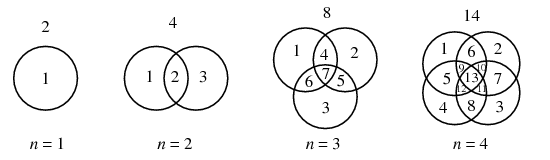
\includegraphics[scale=0.75]{circle.png}
	\end{figure}
	\begin{align*}
		\pi_\F(1) = 2 \ \ \  \pi_\F(2) = 4 \ \ \  \pi_\F(3) = 8  \ \ \ \pi_\F(4) = 14
	\end{align*}
	\begin{align*}
		\pi_\F(n) = n^2 - n + 2
	\end{align*}
\end{frame}

\begin{frame}
More examples: \\
	\begin{enumerate}
		\item Lines on a plane $\pi_\F(n) = n^2/2 + n/2 + 1$
		\item Disks on a plane	$\pi_\F(n) = n^2 - n + 2$
		\item Balls in $\R^3$  $\pi_\F(n) = n^3/3 - n^2 + 8n/3$
		\item Intervals on a line $\pi_\F(n) = 2n$
		\item Half-planes on a plane $\pi_\F(n) = n(n+1)/2 + 1$
		\item Finite subsets of $\N$ $\pi_\F(n) = 2^n$
		\item Polygons in a plane $\pi_\F(n) = 2^n$
	\end{enumerate}
\end{frame}

\begin{frame}
	\begin{Theorem} [Sauer-Shelah]
		Shatter function is either $2^n$ or bounded by a polynomial.
	\end{Theorem}
	\begin{Definition}
		Suppose growth of shatter function for $\F$ is polynomial.
		Let $r$ be the smallest real such that 
		\begin{align*}
			\pi_\F(n) = O(n^r)
		\end{align*}
		We define such $r$ to be the vc-density of $\F$, $\vc(\F)$.
		If shatter function grows exponentially, we let the vc-density to be infinite.
	\end{Definition}
\end{frame}


\begin{frame}
	\frametitle{Applications}
	\begin{itemize}
		\item Vapnik�Chervonenkis Theorem in probability
		\item Computability
		\item NIP theories
	\end{itemize}
\end{frame}

\begin{frame}
	\frametitle{Model Theory}
	Model Theory studies definable sets in first-order structures.
	\begin{align*}
		(\Q, 0, 1, +, \cdot, \leq)
	\end{align*}
	\begin{align*}
		\phi(x) = \exists y \ y \cdot y = x
	\end{align*}
	In the structure above $\phi(x)$ defines a set of numbers that are a square.
\end{frame}

\begin{frame}
	\begin{align*}
		(\R, 0, 1, +, \cdot, \leq)
	\end{align*}
	\begin{align*}
		\phi(x) = \exists y \ y \cdot y = x
	\end{align*}
	In the structure above $\phi(x)$ defines the set $[0, \infty)$.
\end{frame}

\begin{frame}
	\begin{align*}
		(\R, 0, 1, +, \cdot, \leq)
	\end{align*}
	\begin{align*}
		\psi(x_1, x_2) = (x_1 \cdot x_1 + x_2 \cdot x_2 \leq 1.5) \wedge (x_1^2 \leq x_2)
	\end{align*}
	This defines a set in $\R^2$.
\end{frame}

\begin{frame}
	We work with families of uniformly definable sets.
	Fix a formula $\phi(x_1 \ldots x_n, y_1, \ldots y_m)$.
	Plug in elements from the model for $y$ variables to get a family of definable sets in $M^n$.
	\begin{align*}
		\F^M_\phi = \curly{\phi(x_1, \ldots, x_n, a_1, \ldots a_n) \mid a_1, \ldots a_n \in M}
	\end{align*}
	Define $\vc^M(\phi)$ to be the vc-density of the family $\F^M_\phi$
\end{frame}

\begin{frame}
	\begin{align*}
		\phi(x_1, x_2, y_1, y_2, y_3) = (x_1 - y_1)^2 + (x_2 - y_2)^2 \leq y_3^2
	\end{align*}
	In structure $(\R, +, \cdot, \leq)$ given $a,b,r \in \R$ the formula $\phi(x_1, x_2, a, b, r)$ defines a disk in $\R^2$ with radius $r$ with center $(a,b)$.
	Thus $\F^\R_\phi$ is a collection of all disks in $\R^2$.
\end{frame}

\begin{frame}
	A model $M$ is said to have NIP property if all uniformly definable families in it have finite $\vc$-density.
	\begin{itemize}
		\item Examples
		\begin{itemize}
			\item $(\R, 0, 1, +, \cdot, \leq)$
			\item $(\C, 0, 1, +, \cdot)$
			\item $(\Q_p, 0, 1, +, \cdot, \mid)$
		\end{itemize}
		\item Non-examples
		\begin{itemize}
			\item $(\Q, 0, 1, +, \cdot)$
			\item Random graph $(V, R)$.
			\item Pseudo-finite fields.
		\end{itemize}
	\end{itemize}
\end{frame}

\begin{frame}
	\frametitle{vc-density in trees}
	Consider structure $(T, \leq)$
\end{frame}

\end{document}